%% \usepackage[utf8]{inputenc}
\documentclass[pdftex, 12pt, a4paper]{report}
\usepackage{newtxtext, newtxmath}
\usepackage[top=3cm, bottom=3cm, left=3.5cm, right=3cm]{geometry}
\usepackage[hidelinks]{hyperref}
\usepackage[pdftex]{graphicx}
\usepackage[portuguese]{babel}
\usepackage{titlesec}
\usepackage{amsmath}
\usepackage{booktabs}
\usepackage{setspace}
\usepackage{csquotes}
\usepackage{tocloft}
\usepackage{parskip}
\usepackage{amsmath}
\usepackage{amsfonts}
\usepackage[sorting=none]{biblatex}
\addbibresource{bib.bib}
\setstretch{1.5}
\setlength{\cftfigindent}{0pt}
\setlength{\cfttabindent}{0pt}
\renewcommand{\cftdotsep}{1}

\title{\uppercase{P2Q1 MAP22010}}
\newcommand\fypcode{SCSE8338}
\author{Gustavo Soares e Pedro Akira Kitayama}
\date{Junho de 2022}

\begin{document}

\setcounter{page}{1}

\pagebreak
\maketitle
\tableofcontents

\titleformat{\chapter}{\normalfont\huge}{\thechapter.}{20pt}{\huge}

\pagebreak
\chapter{Introdução}
O seguinte relatório tem por objetivo analisar e comentar métodos de resolução de equações diferenciais ordinárias a partir de sistemas de discretizações e condições de contorno adequadas para tal. Em particular, será analisada a seguinte EDO:
$$-u''(x) = f(x), x \in (a,b)$$, onde
$$u(x) = e^{cos{x}}, f(x) = (cosx - sin^{2}x)e^{cosx}$$
Haverá também a implementação do algoritmo de solução da equação utilizando a linguagem python e as bibiliotecas necessárias, em especial a biblioteca numpy.

\pagebreak
\chapter{Desenvolvimento}
\section{Condições de Contorno}
No ramo das equações diferenciais ordinárias, as condições de contorno são uma maneira de impor restrições ao problema a fim de obter unicidade na solução. Problemas de valor sobre o contorno são usados em diversos ramos da física, como em equações de onda, além determinação dos modos normais.

Existem diversos tipos de condições de contorno, mas abordaremos sucintamente abaixo as principais condições utilizadas em problemas de matemática aplicada e  física.
\subsection{Condição de Dirichlet}
Aqui, fixa-se os valores assumidos por $u(x)$ nos extremos do intervalo de interesse: $$u(a) = \alpha \in R$$
$$u(b) = \beta \in R$$
\subsection{Condição de Neumann}
Nesta condição fixa-se o valor da deriva primeira de u (em problemas de física, corresponde ao fluxo do campo estudado) em um dos extremos ou no interior do intervalo $(a,b)$.
\subsection{Condição de Robin}
Também chamada de condição de contorno de Fourier, impõe em uma equação diferencial ordinária uma relação linear entre os valores da função e os valores da derivada da função na fronteira do domínio, isto é, nada mais é que uma combinação linear das condições de Dirichlet e Neumann.
\section{Escolhendo a condição de fronteira}
Para a EDO estudada, será utilizada uma condição de contorno de dirichlet sobre os extremos do intervalo $(0,2\pi)$:
$$u(0) = u(2\pi) = e$$
\section{Escolhendo o modelo de discretização}
Para discretizar essa EDO estaremos utilizando em conjunto os sistemas de discretização (2) e (5) fornecidos no enunciado:

$$
       \begin{cases}

            u_{k-1} - u_{k} + u_{k+1} = -f_{k}h^{2}, & \mbox{se }i = 1  \mbox{,} n-1 \\

             -u_{k-2} + 16u_{k-1} -30u_{k} + 16u_{k+1} - u_{k+2} = -12h^{2}f_{k}, & \mbox{caso contrário.}

       \end{cases}
$$

O primeiro sistema possui erro da ordem de $O(h^{2})$ enquanto que o segundo $O(h^{4})$, logo como utilizaremos um n suficiente alto, é esperado  que o erro empírico do método convirja para $p = 4$, pois apenas os dois pontos extremos foram discretizados com $p=2$.

\section{Forma do sistema linear}
Então, aplicando os métodos de discretização citados, o sistema linear Ax = b resultante foi:

\[
\begin{bmatrix}
    -2 & 1 & &  & \\
    16 & -30 & 16 & -1& && \\
    -1 & 16 & -30  & 16 & -1 \\
     & -1 & 16 &-30&16&-1\\
    &      &  \ddots & \ddots &\ddots&\ddots&\ddots\\
    &       &         & -1&16&-30&16&-1\\
    &       &         &   & -1& 16&-30&16\\
    &       &         &   &   &   & 1& -2
\end{bmatrix}  
\begin{bmatrix}
    u_1 \\
    u_2 \\
    \vdots \\
    u_{n-1}
\end{bmatrix}
    = 
\begin{bmatrix}

    -f_1\cdot h^{2} - u_0 \\
    -12f_2\cdot h^{2} + u_0\\
    -12f_3\cdot h{2} \\
    \vdots\\
    -12f_k\cdot h^{2}h\\
    \vdots\\
    -12f_{n-2}\cdot h^{2} + u_6\\
    -f_{n-1}\cdot h^{2}-

\end{bmatrix}
\]

Note que A é uma matriz de banda (e esparsa). Isso traz uma propriedade em particular que é interessante, que é o pouco uso de memória já que só é necessário armazenar os elementos diferentes de zero da matriz. Assim, um método bem eficiente encontrado para resolver a matriz é com a função spsolve do módulo de resolução de álgebra linear da biblioteca scipy (scipy.sparse.linalg).

\section{Verificando a qualidade da solução}
Uma etapa importante é verificar se a solução obtida faz sentido gráficamente, comparando os pontos gerados pelo método com o gráfico da solução exata, essa é o cerne do conceito da verificação por solução manufaturada. Para isso, por meio da biblioteca matplotlib geramos essa comparação para alguns valores de $n$, obtendo:

\begin{figure}[ht]
    \centering
    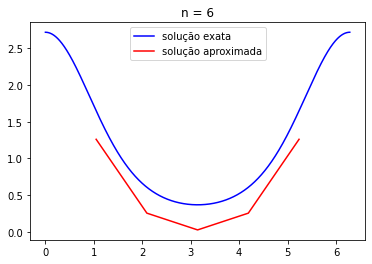
\includegraphics[scale = 0.8]{n=6.png}
    \caption{Comparação com n = 6}
    \label{fig:my_label}
\end{figure}

\begin{figure}[ht]
    \centering
    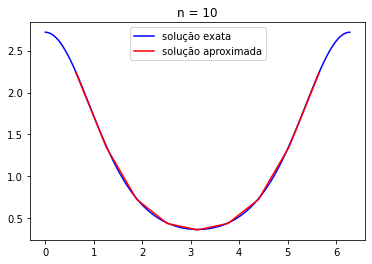
\includegraphics[scale = 0.8]{n=10.png}
    \caption{Comparação com n = 10}
    \label{fig:my_label}
\end{figure}

\begin{figure}[ht]
    \centering
    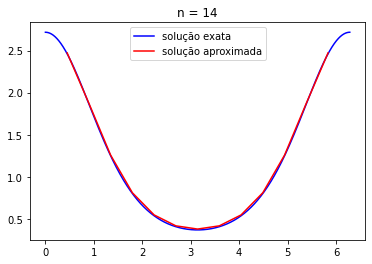
\includegraphics[scale = 0.8]{n=14.png}
    \caption{Comparação com n = 14}
    \label{fig:my_label}
\end{figure}

\begin{figure}[ht]
    \centering
    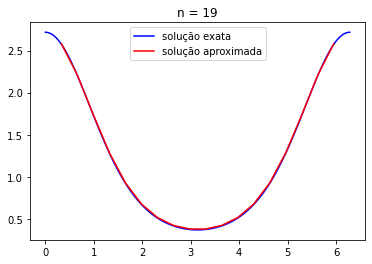
\includegraphics[scale = 0.8]{n=19.png}
    \caption{Comparação com n = 19}
    \label{fig:my_label}
\end{figure}
\chapter{Conclusão}
\section{Resultados}
A tabela de resultados para norma-2 ficou da seguinte forma:
\begin{table}[ht]
\begin{tabular}{@{}llll@{}}
\toprule
$n$  & $h = \frac{(b - a)}{n}$ & $ \left\| e(h) \right\| =  \left\| u - \eta(h)\right\|$ & $p = \log_{2}(\left\| e(h) \right\|/\left\| e(h/2) \right\|)$ \\ \midrule
128  & $4.90873852 \cdot 10^{-1}$  & $5.99908552 \cdot 10^{-5}$                                  &                                                               \\
256  & $2.45436926 \cdot 10^{-2}$  & $5.37533254 \cdot 10^{-6}$                                  & 3.480316683                                                   \\
512  & $1.227118463 \cdot 10^{-2}$ & $4.77121751 \cdot 10^{-7}$                                  & 3.493924646                                                   \\
1024 & $6.135923151 \cdot 10^{-3}$ & $4.22558422 \cdot 10^{-8}$                                  & 3.497134733                                                   \\
2048 & $3.067961576 \cdot 10^{-3}$ & $4.04241007 \cdot 10^{-9}$                                  & 3.385863236                                                   \\
4096 & $1.533980788 \cdot 10^{-3}$ & $3.08815297 \cdot 10^{-9}$                                  & 0.388471461                                                   \\ \bottomrule
\end{tabular}
\end{table}

E a tabela para norma do máximo ficou:
\begin{table}[ht]
\begin{tabular}{@{}llll@{}}
\toprule
$n$  & $h = \frac{(b - a)}{n}$ & $ \left\| e(h) \right\| =  \left\| u - \eta(h)\right\|$ & $p = \log_{2}(\left\| e(h) \right\|/\left\| e(h/2) \right\|)$ \\ \midrule
128  & $4.90873852 \cdot 10^{-1}$  & $5.97365577 \cdot 10^{-6}$                                  &                                                               \\
256  & $2.45436926 \cdot 10^{-2}$  & $3.79391701 \cdot 10^{-7}$                                  & 3.976854078                                                   \\
512  & $1.227118463 \cdot 10^{-2}$ & $2.38103564 \cdot 10^{-8}$                                  & 3.994027003                                                   \\
1024 & $6.135923151 \cdot 10^{-3}$ & $1.49008672 \cdot 10^{-9}$                                  & 3.998121012                                                   \\
2048 & $3.067961576 \cdot 10^{-3}$ & $9.413581 \cdot 10^{-11}$                                  &  3.984508842                                                  \\
4096 & $1.533980788 \cdot 10^{-3}$ & $6.22437102 \cdot 10^{-9}$                                  & 0.596815586                                                   \\ \bottomrule
\end{tabular}
\end{table}

\end{document}
